% This must be in the first 5 lines to tell arXiv to use pdfLaTeX, which is strongly recommended.
\pdfoutput=1
% In particular, the hyperref package requires pdfLaTeX in order to break URLs across lines.

\documentclass[11pt]{article}

% Remove the "review" option to generate the final version.
\usepackage[review]{ACL2023}

% Standard package includes
\usepackage{times}
\usepackage{latexsym}

% For proper rendering and hyphenation of words containing Latin characters (including in bib files)
\usepackage[T1]{fontenc}
% For Vietnamese characters
% \usepackage[T5]{fontenc}
% See https://www.latex-project.org/help/documentation/encguide.pdf for other character sets

% This assumes your files are encoded as UTF8
\usepackage[utf8]{inputenc}

% This is not strictly necessary, and may be commented out.
% However, it will improve the layout of the manuscript,
% and will typically save some space.
\usepackage{microtype}

% This is also not strictly necessary, and may be commented out.
% However, it will improve the aesthetics of text in
% the typewriter font.
\usepackage{inconsolata}
\usepackage{enumitem}

% If the title and author information does not fit in the area allocated, uncomment the following
%
%\setlength\titlebox{<dim>}
%
% and set <dim> to something 5cm or larger.

\title{Zero Shot Task Oriented Dialog}

% Author information can be set in various styles:
% For several authors from the same institution:
% \author{Author 1 \and ... \and Author n \\
%         Address line \\ ... \\ Address line}
% if the names do not fit well on one line use
%         Author 1 \\ {\bf Author 2} \\ ... \\ {\bf Author n} \\
% For authors from different institutions:
% \author{Author 1 \\ Address line \\  ... \\ Address line
%         \And  ... \And
%         Author n \\ Address line \\ ... \\ Address line}
% To start a seperate ``row'' of authors use \AND, as in
% \author{Author 1 \\ Address line \\  ... \\ Address line
%         \AND
%         Author 2 \\ Address line \\ ... \\ Address line \And
%         Author 3 \\ Address line \\ ... \\ Address line}

\author{First Author \\
  Affiliation / Address line 1 \\
  Affiliation / Address line 2 \\
  Affiliation / Address line 3 \\
  \texttt{email@domain} \\\And
  Second Author \\
  Affiliation / Address line 1 \\
  Affiliation / Address line 2 \\
  Affiliation / Address line 3 \\
  \texttt{email@domain} \\}

\begin{document}
\maketitle
\begin{abstract}
  This document is a supplement to the general instructions for *ACL authors. It contains instructions for using the \LaTeX{} style file for ACL 2023.
  The document itself conforms to its own specifications, and is, therefore, an example of what your manuscript should look like.
  These instructions should be used both for papers submitted for review and for final versions of accepted papers.
\end{abstract}


\section{Introduction}


\section{Methodology}

\subsection{Problem Formulation}

A dialog session is composed of multiple turns, which consists of interactions between the user and the system
in natural language utterance.
The SGD dataset provides a list of Schemas, $S = (s_1, ...., s_n)$ and each dialog contains a list of service names, which
can be used to extract the relevent schema for that dialog, $S_r \in S$.

For a turn $t$, the inputs to the model are the following: user utterance $U_t$, DST from the previous turn $D_{t-1}$, relevant schemas $S_r$, database search results $Db_t$
and a list of system action names $Action_{all}$.
The model autoregressively generates the dialog state $D_{t}$, user actions $UA_t$, system actions $SA_t$ and system response $R_t$.
Figure~\ref{fig:our_model} shows a visual representation of the overall approach.

A dialog session is composed of multiple interactions between a user and a system in natural language utterance.
At turn $t$, the user utters $U_t$ and the system responds with $S_t$. In a multi-domain dialog system with $m$ domains, the domain
knowledge is encapsulated in a schema, $Schema_i \in Schema = \{Schema_1, ..., Schema_m\}$.
A schema object, $Schema_i$, contains the domain name, a list of slots
Our model~\oursys, at timestep $t$ estimates the probability of the dialog state at $D_t$ as follows:

\begin{equation}
    P(D_t | U_t, D_{t-1}, Schema_i)
    \label{eq:dialog_state}
\end{equation}

The dialog state consists of a triplets of slot names and values from domain $i$, $D_t = \{S^i_1, ..., S^i_n\}$.

\subsection{Input and Output Representation}

\textbf{Should I write about this?}

\subsection{Training}

A GPT model is passed an input prompt and the model generates a response based on this. The input prompt is contained
in the response of the model.
Let $t_1, ..., t_p$ be the tokens in the input prompt and $t_{p+1}, ..., t_{n}$ be the tokens in the response.
While optimizing a GPT model, the common practice is to calculate the Cross Entropy (CE) loss on the full sequence, $t_1, ..., t_n$.

In this paper, we propose a two step training approach for training TOD systems that use generation models.
In the first step, we follow the standard training procedure and calculate the CE loss on the full sequence, $t_1, ..., t_n$.
For the second step, we intialize the model with the weights from the first step and calculate the CE loss only on the response,
as shown in Equation~\eqref{eq:loss_func}.

\begin{equation}
    L = - \sum_{i=p+1}^{n} t_i \log(p_i)
    \label{eq:loss_func}
\end{equation}

Formulating the loss in this way ensures that in turns that have a long input prompt, the model will not get an extra
reward for generating the prompt, rather the full focus would be on optimizing the response.

\section{Experimental Setup}

\subsection{Datasets}

\textbf{The Schema Guided Dialogue (SGD)} dataset is a large scale dataset for task oriented dialogue that consists of over 16K multi domain
dialogs between a human and a virtual assistant covering 16 domains. The dataset also provides a schema for each domain that
provides a textual description of the domain, list of slots and list of intents. A slot contains a name, textual description,
and possible values for categorical slots and an intent contains a name, textual description, optional slots and result slots.

\textbf{SGD-X} dataset is an extension of the SGD dataset that contains that contains stylistic variants for every schema in SGD.
It provides 5 variants of schemas, where each variant incrementally moves further away from the original schema.
The goal of this dataset is to evaluate model sensitivity to schema variations,
and the authors of the dataset have shown that two of the top performing schema guided DST models are sensitive to schema changes and have had significant performance drops on SGD-X.

\subsection{Evaluation Metrics}

To evaluate the performance of our model, we compute multiple metrics on each component of the TOD system.

\textbf{DST.} We evaluate the performance DST by calculating the Intent Accuracy, Average Goal Accuracy, Joint Goal Accuracy and Requestes Slot F1, all of which
are suggested by the SGD dataset. Since the SGD dataset was created for evaluating DST, it does not contain metrics for evaluating system
actions and response.

\textbf{System Actions.} To evaluate the system actions, we compute the metrics Inform, Success, Average Action Accuracy (AAA) and Joint Action Accuracy (JAA).
Inform measures whether a system has provided a correct entity and Success measures whether it has answered all the requested
information. AAA and JAA are similar to the goal metrics in SGD, but are calculated from system actions. Since we predict user actions, we calcuate the
average and joint accuracy of the predicted user actions.

\textbf{System Response.} For evaluating the system response, we report the GLEU~\cite{wu2016googles} score as it performs better on individual sentence pairs.

\textbf{Overall.} To get an overall score for the model, we calculate the combined score~\cite{mehri2019structured}: (Inform + Success) $\times$ 0.5 + GLEU.

Since the SGD dataset does not contain any metrics for system actions, we had to implement the following metrics: Inform, Success, AAA and JAA;
to evaluate the performance of system actions.
For inform, from the ground truth system actions we filter actions by action type inform (Inform, Inform Count)
and check if they are predicted correctly. For success, we filtere actions by slot names that are in the requested slots and
check if the action slot values are predicted correctly. AAA and JAA are implemented following the implementations of AGA and JGA.
To ensure a fair comparison of~\oursys~with existing systems that have reported results on the SGD dataset,
we use the evaluation script provided by the SGD dataset.





\begin{table*}
    \centering
    \begin{adjustbox}{max width=\textwidth}
        \begin{tabular}{|c|c|c|c|c|c|c|c|c|c|c|c|c|}
            \hline
            \multirow{3}{*}{Model}    &         & \multirow{2}{*}{Intent}   & Requested & Average        & Joint          &                &         & Average  & Joint    & \multirow{2}{*}{Response} &          \\
                                      & Domains & \multirow{2}{*}{Accuracy} & Slots     & Goal           & Goal           & Inform         & Success & Action   & Action   & \multirow{2}{*}{GLEU}     & Combined \\
                                      &         &                           & F1        & Accurracy      & Accuracy       &                &         & Accuracy & Accuracy &                           &          \\ \hline
            \multirow{3}{*}{\oursys~} & all     & 84.83                     & 95.53     & \textbf{72.38} & \textbf{48.44} & \textbf{73.08} & 62.19   & 58.32    & 46.31    & 20.04                     & 87.67    \\
                                      & seen    & 85.48                     & 95.88     & \textbf{74.23} & \textbf{52.05} & \textbf{74.72} & 63.85   & 60.19    & 48.69    & 24.66                     & 93.95    \\
                                      & unseen  & 84.45                     & 95.42     & \textbf{72.03} & \textbf{47.83} & \textbf{71.68} & 61.63   & 57.42    & 45.21    & 18.51                     & 85.16    \\ \hline
            {w/o}                     & all     & 75.08                     & 92.80     & 62.47          & 39.52          & 48.13          & 44.27   & 40.38    & 30.71    & 11.41                     & 57.61    \\
            {Two Step}                & seen    & 75.75                     & 93.13     & 64.66          & 42.76          & 50.26          & 46.47   & 41.96    & 32.42    & 13.75                     & 62.11    \\
            {Training}                & unseen  & 75.79                     & 92.90     & 62.60          & 39.25          & 47.55          & 44.32   & 40.25    & 30.66    & 11.03                     & 56.97    \\ \hline
            {w/o}                     & all     & 83.14                     & 94.67     & 64.70          & 38.47          & 59.88          & 53.88   & 54.14    & 43.07    & 21.15                     & 78.03    \\
            {Domain}                  & seen    & 84.34                     & 95.10     & 67.62          & 43.39          & 62.30          & 56.64   & 56.61    & 45.92    & 27.10                     & 86.57    \\
            {Schema}                  & unseen  & 82.96                     & 94.52     & 63.95          & 37.59          & 58.65          & 53.25   & 53.22    & 42.20    & 19.33                     & 75.28    \\ \hline
            % {w/o}                  & all     & 88.22                     & 95.72     & 71.51          & 42.68          & 64.15          & 60.98   & 57.34    & 45.26    & 20.70                     & 83.27    \\
            % {User}                 & seen    & 89.02                     & 96.07     & 73.86          & 47.02          & 65.80          & 63.17   & 59.48    & 47.83    & 25.96                     & 90.44    \\
            % {Actions}              & unseen  & 87.94                     & 95.59     & 71.05          & 41.78          & 63.09          & 60.73   & 56.46    & 44.41    & 18.82                     & 80.73    \\ \hline
            {w/o}                     & all     & 87.50                     & 95.48     & 71.54          & 43.20          & 50.96          & 56.89   & 53.67    & 41.73    & 17.62                     & 71.54    \\
            {DB}                      & seen    & 88.26                     & 95.85     & 73.87          & 47.62          & 53.03          & 59.08   & 55.73    & 43.91    & 23.12                     & 79.17    \\
            {Results}                 & unseen  & 87.19                     & 95.36     & 71.04          & 42.17          & 50.33          & 56.95   & 53.17    & 41.52    & 16.07                     & 69.70    \\ \hline
            {w/o Sys}                 & all     & 87.56                     & 96.00     & 72.86          & 44.52          & 60.13          & 61.91   & 57.98    & 45.86    & 21.02                     & 82.04    \\
            {Action}                  & seen    & 88.25                     & 96.32     & 75.11          & 48.77          & 61.69          & 64.04   & 60.12    & 48.37    & 26.56                     & 89.43    \\
            {Names}                   & unseen  & 87.38                     & 95.91     & 72.44          & 43.60          & 59.61          & 61.75   & 57.29    & 45.26    & 19.16                     & 79.84    \\ \hline
        \end{tabular}
    \end{adjustbox}
    \caption{Ablation Study of~\oursys.}
    \label{tab:ablation-results}
\end{table*}

\section{Results}
\begin{table}
    \begin{adjustbox}{max width=0.45\textwidth}
        \begin{tabular}{|c|c|c|c|c|}
            \hline
            \multirow{2}{*}{Model} & Intent   & Requested & Average & Joint \\
                                   & Accuracy & Slot F1   & GA      & GA    \\ \hline
            SGD Baseline           & 90.60    & 96.50     & 56      & 25.40 \\ \hline
            FastSGT                & 90.33    & 96.33     & 60.66   & 29.20 \\ \hline
            Seq2Seq-DU             & 91.00    & -         & -       & 30.10 \\ \hline
            DSGFNET                & -        & -         & -       & 32.10 \\ \hline
            \oursys~               & 81.49    & 95.97     & 74.08   & 49.73 \\ \hline
        \end{tabular}
    \end{adjustbox}
    \caption{Results on SGD test set. Our approach significantly outperforms baselines methods in terms of average and joint goal accuracy.}
    \label{tab:other-results}
\end{table}

Since there are no End-to-End TOD systems for the SGD dataset, we re-implemented some of the popular baseline methods to
compare with our approach and present the results in Table~\ref{tab:main-results}.

We can see that~\oursys~outperforms all the baselines across all metrics except GLEU. An explanation of this could be that since we
replaced the dialog history with the dialog state, the model lost a lot of exposure to dialog utterances.
Another reason could be that, while the system response requires a fluent generation, all other parts of the generation can be deemed as a structured generation.
A greedy decoding strategy generally works well for structured generation, but is not the best strategy for fluent generation, whereas
nucleus and top-k sampling strategies are better suited for fluent generation, but are not the best for structured generation.
We formulated the problem as a single sequence generation, and we can only select one strategy, so there is bound to be a trade-off since
there is no one strategy that is best suited for both fluent and structured generation.
We opted to use greedy decoding, which may have been the cause for the loss of fluency in the response generation.

We evaluate the DST performance of~\oursys~with the evaluation script provided by the SGD dataset and present our results alongside
other baseline DST models in Table~\ref{tab:other-results}.
We can see that even though our method is not specifically designed for DST, still it significantly outperforms the baselines models in the
important metrics: Average and Joint Goal Accuracy.

\subsection{Long Range Dialog Dependencies}

\begin{figure}[t]
    \centering
    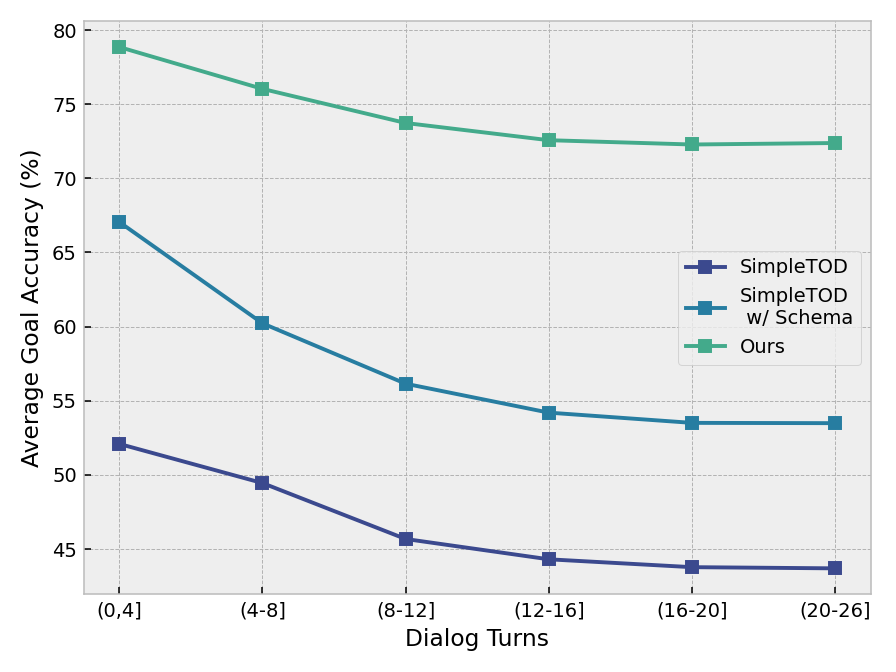
\includegraphics[width=\linewidth]{assets/dialog_turns.png}
    \caption{
        Performance of dialog systems on the SGD test set with respect to dialog turns
    }
    \label{fig:dialog_turns}
\end{figure}

In order to process dialogs that have a large number of turns, a system must be effective at capturing long range dependencies.
To test this ability, we group the test dialogs based on the number of turns and evaluate the performance of~\oursys~and a few baseline systems on each group.
As shown in Figure~\ref{fig:dialog_turns},~\oursys~outperforms the baseline systems across all groups.

Generally, in the first few turns of a dialog, the main focus is on figuring out what the user wants. The user could switch before mulitple options before finally deciding on one, however
towards the end of a dialog, usually the user has a clear idea of what they want, so he or she is less likely to make many changes.
For the first few turns, we have observed that there is a steeper drop in performance of the baseline when compared to~\oursys~.
A possible explanation of this could be that, since we pass the dialog summary to the model, it contains the correct state of the dialog at the previous turn, which helps the model to make better predictions.
Whereas in the baseline system, the model has to infer the previous state from the dialog history, which is a more difficult task.
In groups with large number of turns, both the baseline and~\oursys~perform similarly, which suggests even though~\oursys~does well in capturing
medium range dependencies, long range dependencies are still a challenge for the model.


\subsection{Two Step Training}

\begin{figure}[t]
    \centering
    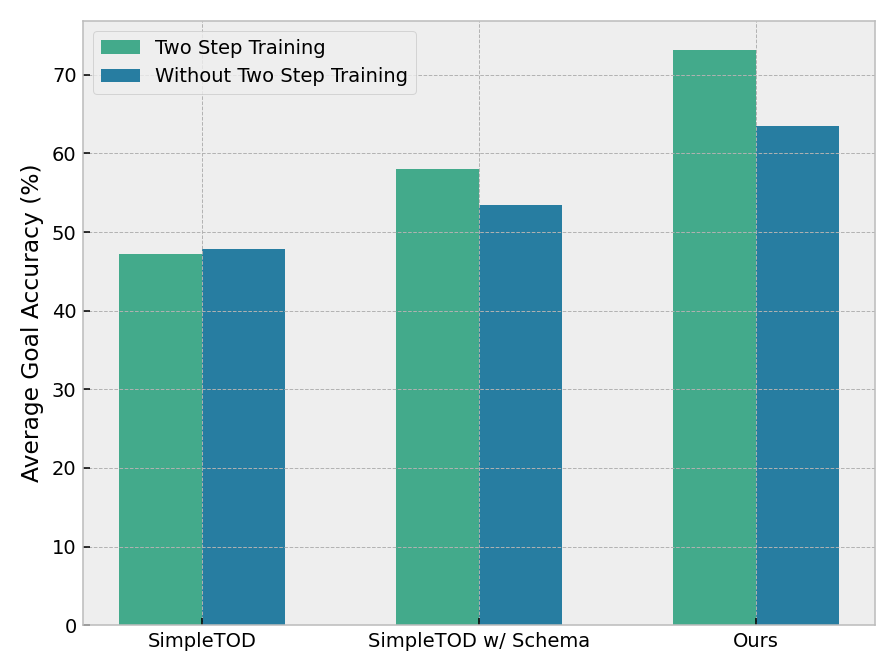
\includegraphics[width=\linewidth]{assets/two_step_training.png}
    \caption{
        Effect of Two Step Training on dialog systems
    }
    \label{fig:two_step_training}
\end{figure}

To better understand the effect of the two step training process, we compared~\oursys~and a few baseline systems with and without the two step training process.
In Figure~\ref{fig:two_step_training}, we can see that models that incorporate schema benefit from the two step training process.
\textbf{I am unable to come up with a solid explanation for why this happens, maybe you can think of something.}

\subsection{Ablation Study}

To get a better understanding of the different components of our model, we drop a certain component of~\oursys~to show effect on the performance
and report an ablation study in Table~\ref{tab:ablation-results}.
We can see that dropping two step training drastically degrades performance across all metrics, which suggests the importance of the training mechanism for~\oursys.

The role of schema is also important as we can see that the performance of~\oursys~drops across all metrics when we drop schema.
Another important aspect to notice here is that this variant has the largest difference in performance between seen and unseen domains.
These observations indicate that schema not only aids the model to generalize to new domains, but also plays a central role in the overall performance of the system.

\textbf{Write this section after experiments finish}We can observe that removing database results has a large impact on the metrics related to system actions.
We can see that removing list of system actions has decreased the metrics related to system actions, particularly Inform.
However, there is no significant decrease in metrics related to DST and system response. Database results have some correlation with DST,
so these components have a larger effect on DST when compared to list of system actions. As expected, the major drop in performance occurs when we
elect to drop schema. Not only does the performance drops significantly in the unseen domain, there is also a performance degradation
across all other metrics by a noticeable amount. This shows that schema is an important component in our approach as
it not only helps the model to generalize to new domains, but also plays a crucial role in the overall performance of the system.






\subsection{SGD-X}
% \begin{table*}
%     \centering
%     \begin{adjustbox}{max width=\textwidth}
%         \begin{tabular}{|c|c|c|c|c|c|c|c|c|c|c|c|c|}
%             \hline
%             \multirow{3}{*}{Model} & \multirow{2}{*}{Intent}   & Requested   & Average     & Joint       &            &             & Average     & Joint       & \multirow{2}{*}{Response} &              \\
%                                    & \multirow{2}{*}{Accuracy} & Slots       & Goal        & Goal        & Inform     & Success     & Action      & Action      & \multirow{2}{*}{GLEU}     & Combined     \\
%                                    &                           & F1          & Accurracy   & Accuracy    &            &             & Accuracy    & Accuracy    &                           &              \\ \hline
%             \oursys~               & 55.63, 7.7                & 89.67, 0.29 & 50.23, 3.84 & 29.46, 1.31 & 38.90, 2.9 & 26.47, 2.62 & 38.03, 2.12 & 33.60, 1.37 & 15.60, 0.91               & 48.29, 3.53  \\ \hline
%             SimpleTod w/ Schema    & 23.37, 6.03               & 88.23, 1.42 & 19.99, 4.29 & 10.75, 2.89 & 28.76, 7.7 & 16.21, 6.79 & 28.21, 5.2  & 24.19, 4.4  & 14.14, 3.39               & 36.62, 10.14 \\ \hline
%         \end{tabular}
%     \end{adjustbox}
%     \caption{SGD-x results on unseen domain. The mean and standard deviation across all 5 versions is reported for each metric}
%     \label{tab:sgdx-results}
% \end{table*}



\begin{figure}[t]
    \centering
    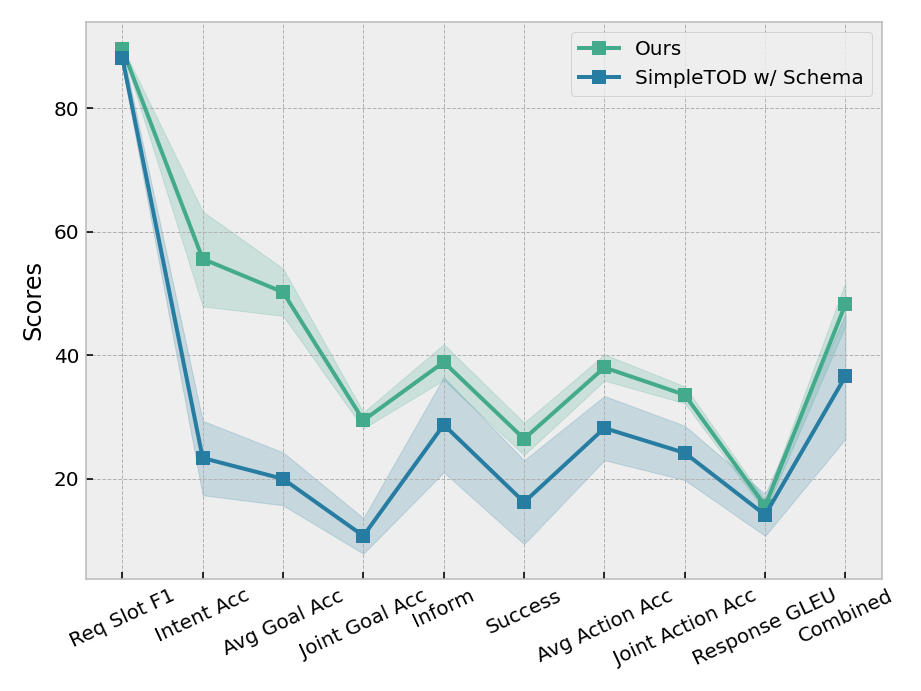
\includegraphics[width=\linewidth]{assets/sgdx_results.png}
    \caption{
        SGD-X results: For the 5 versions of SGD-X, we plot the mean of each metric and represent the standard deviation as the shaded area.
    }
    \label{fig:sgdx_graph}
\end{figure}



To access the robustness of~\oursys, we ran experiments on the unseen domains of the SGD-X dataset and the results are presented in Figure~\ref{fig:sgdx_graph}.
The line graph shows the mean of each metric across all 5 versions of SGD-X and the shaded area represents the standard deviation.
At first glance, we can see that the baseline has a much larger standard deviation than~\oursys~and upon a closer inspection, we can see that
there is more variation in metrics that evaluate the system actions: Inform, Success, AAA and JAA.
For~\oursys, we can see DST metrics have a larger standard deviation, which could be due to the fact that~\oursys~has a low Intent Accuracy metric
than other DST models as shown already in Table~\ref{tab:other-results}. \textbf{Is this too negative? Should I drop this?}





\section{Related Works}



\subsection{Supervised End to End Models}
Pretrained language models like BERT~\cite{Devlin2019BERTPO}, GPT-2~\cite{Radford2019LanguageMA} and T5~\cite{Raffel2019ExploringTL}
have been used extensively in the literature for End to End models for TOD systems~\cite{HosseiniAsl2020ASL,Peng2021SoloistBT,Lee2020SUMBTLaRLEN,Yang2020UBARTF,Jeon2021DORATP,Sun2022BORTBA,Yang2022UBARv2TM,Noroozi2020AFA}.
In these models, the context consists of the dialog history, whereas our approach uses the last user utterance and the previous state DST as context.
Moreover, most of these models have the best performance in supervised settings and do not generalize well to unseen domains.

\subsection{Zero Shot Dialog Models}

Recently, some work has been done on Zero Shot generalizability by incorporating schema to transfer knowledge across domains, however these systems
only focus on certain components of TOD systems, such as for DST~\cite{Feng2020ASA,Feng2022DynamicSG,Lee2021DialogueST,Noroozi2020AFA,Wang2022SlotDM}
and next action prediction and response generation~\cite{Mosig2020STARAS,Mehri2021SchemaGuidedPF}.
However, in this paper, we propose an End-to-End TOD system that is Zero-Shot generalizable.

\textbf{write about prompt based systems}



% Entries for the entire Anthology, followed by custom entries
\bibliography{anthology,custom}
\bibliographystyle{acl_natbib}

\appendix

\section{Example Appendix}
\label{sec:appendix}

This is a section in the appendix.

\end{document}
